\newif\iffull\fullfalse% do not change flags here
\newif\ifdraft\draftfalse% do not change flags here

\fulltrue  % full  = long version (stuff to move to appendix)
\drafttrue % draft = comments and half-baked bits

%\pdfsuppressptexinfo-1

%
%\documentclass[letterpaper,table,dvipsnames,10pt]{article}
\documentclass[hyperref,envcountsame,envcountsect,runningheads]{llncs}%
\usepackage[dvipsnames]{xcolor}
\usepackage{hyperref}
% \pagestyle{plain}
%   \addtolength{\oddsidemargin}{-.5in}
%   \addtolength{\evensidemargin}{-.5in}
%   \addtolength{\textwidth}{1in}
\hypersetup{
    bookmarks=true,         % show bookmarks bar?
    unicode=false,          % non-Latin characters in Acrobat�s bookmarks
    colorlinks=true,       % false: boxed links; true: colored links
    linkcolor=RoyalPurple,          % color of internal links (change box color with linkbordercolor)
    citecolor=black,
    filecolor=black,
    urlcolor=black,
    hypertexnames=false
}
 \pagestyle{plain}
%   \addtolength{\oddsidemargin}{-1.6in}
%   \addtolength{\evensidemargin}{-1.6in}
%   \addtolength{\textwidth}{3.2in}

\def\topfraction{0.8}

\setcounter{tocdepth}{2}

%\usepackage{savetrees}
\usepackage{xspace}
\usepackage{lmodern}
\usepackage[utf8]{inputenc}
\usepackage[T1]{fontenc}
\usepackage[english]{babel}
\usepackage{latexsym}
\usepackage{amsmath,amsfonts,amssymb}
\usepackage{nameref}
%\usepackage{cleveref}
%\usepackage{amsthm}
\usepackage{tikz}
\usetikzlibrary{fit}

\usepackage{verbatim}
\usepackage{enumitem}
\usepackage[probability,adversary,sets,operators,primitives]{cryptocode}[=2018-11-11]
\usepackage{wrapfig}
\usepackage{booktabs}
\usepackage{pdfpages}
\usepackage{enumitem}
\usepackage{multicol}
\usepackage{catchfilebetweentags}
% \usepackage{lipsum}
\usepackage{url}
\usepackage{lscape}
\usepackage{subcaption}
\usepackage{todonotes}
\usepackage{placeins}
\usepackage{rotating}
\usepackage{thm-restate}

%\makeatletter
%\let\claim\@undefined
%\let\endclaim\@undefined
%\makeatother
%\spnewtheorem{claim}[theorem]{Claim}{\bfseries}{\itshape}

% include code in verbatim
\usepackage{listings}
\lstset{basicstyle=\footnotesize\ttfamily,
breaklines=true,
numbers=left,
tabsize=4,
escapeinside={<@}{@>}}

\let\llncssubparagraph\subparagraph
\let\subparagraph\paragraph
\usepackage{titlesec}
%\let\subparagraph\llncssubparagraph
\let\paragraph\subsubsection
\titlespacing*{\section} {0pt}{3ex plus 1ex minus .2ex}{2.1ex plus .2ex}
\titlespacing*{\subsection} {0pt}{2.75ex plus 1ex minus .2ex}{1.3ex plus .2ex}
\titlespacing*{\subsubsection}{0pt}{1ex plus 1ex minus .2ex}{2mm}

\newcommand{\ADM}{\text{\textrm{\upshape ADM}}}
\newcommand{\StyleModel}[1]{\V{{#1}}}
\newcommand{\StyleKey}[1]{\ensuremath{\mathit{#1}}}

\renewcommand{\lll}{\text{left}}
\newcommand{\rrr}{\text{right}}
\newcommand{\mmm}{\text{middle}}
\newcommand{\XPN}{\n{XPN}}
\newcommand{\XTN}{\n{XTN}}


\newcommand{\hon}{\V{{hon}}}
\newcommand\admid{\n{admid}}
\newcommand\idx{\O{idx}}
\newcommand\ctr{\n{ctr}}
\newcommand\ks{\n{ks}}

\newcommand{\ksc}{\mathsf{ksc}}
\renewcommand{\vec}[1]{\textbf{#1}}

\newcommand{\outputof}{\mathsf{output}}
\newcommand{\vecgets}{\stackrel{\textbf{vec}}{\gets}}
\newcommand{\choosegets}{\stackrel{\text{choose}}{\gets}}
\newcommand{\cequiv}{\stackrel{\textbf{code}}{\equiv}}
\newcommand{\vecequal}{\stackrel{\textbf{vec}}{=}}


\newcommand{\GKG}{\M{GKG}}
\newcommand{\cnt}{\textsf{cnt}}
\renewcommand{\H}{\textsf{H}}
\newcommand{\RO}{\textsf{RO}}
\newcommand{\RPO}{\textsf{RPO}}
\newcommand{\E}{\textsf{E}}
\newcommand{\ininterface}[1]{{[\M{#1}\rightarrow]}} %{I^{in}_{#1}}
\newcommand{\outinterface}[1]{{[\rightarrow\M{#1}]}} %{I^{out}_{#1}}
\newcommand{\V}[1]{\ensuremath{\mathit{#1}}}

\newcommand{\args}{\StyleModel{args}}
\newcommand{\history}{\StyleModel{history}}
\newcommand{\Handles}{\vec h}
\newcommand{\Keys}{\vec k}
\renewcommand{\hash}{\O{hash}}
\newcommand{\xtr}{\O{xtr}}
\renewcommand{\dh}{\O{dh}}
\newcommand{\hmac}{\O{xtr}}
\renewcommand{\prf}{\hmac}
\newcommand{\xpd}{\O{xpd}}
\newcommand{\hkdf}{\O{xpd}}
\newcommand{\dkdf}{\O{kdf}}
\newcommand{\kdf}{\hkdf}
\newcommand{\gendh}{\O{gendh}}
\newcommand{\honest}{\mathsf{honest}}
\newcommand{\honestShares}{\mathsf{honestShares}}

\newcommand{\ReturnHandles}{\StyleModel{ReturnHandles}}
\newcommand{\CompHand}{\O{CompHand}}
\newcommand{\CompInput}{\O{CompInput}}
\newcommand{\CompKey}{\O{CompKey}}
\newcommand{\compK}[1]{\mathsf{nextKeys}(#1)}
\newcommand{\CompKeys}{\CompKey}
\newcommand{\lastShares}{\mathsf{shares}}
\newcommand{\lastPsk}{\mathsf{psk}}
\newcommand{\level}{\mathsf{level}}
\newcommand{\sort}{\mathsf{sort}}
\newcommand{\length}{\mathsf{len}}
\newcommand{\outlen}{\length}
\newcommand{\keylen}{\length}
\newcommand{\esalt}{\StyleModel{esalt}}
\newcommand{\share}{\StyleModel{share}}
\newcommand{\localshare}{X}% or \share_\local
\newcommand{\peershare}{Y}% or \share_\peer
\newcommand{\exponent}{\StyleModel{exp}}
\newcommand{\shares}{\StyleModel{shares}}
\renewcommand{\th}{\StyleModel{th}}
%\renewcommand{\dh}{\StyleModel{dh}}
\newcommand{\hs}{\StyleModel{hs}}
\newcommand{\bind}{\StyleModel{bind}}
\newcommand{\eem}{\StyleModel{eem}}
\newcommand{\es}{\StyleModel{es}}
\newcommand{\cet}{\StyleModel{cet}}
\newcommand{\cekey}{\StyleModel{cekey}}
\newcommand{\ceiv}{\StyleModel{ceiv}}
\newcommand{\Label}{\lbl{label}}
\newcommand{\ctx}{\V{ctx}}
\newcommand{\isres}{\StyleModel{is}\_\StyleModel{res}}

\newcommand{\stack}[1]{{\scriptsize\begin{array}{l} #1 \end{array}}}
\newcommand*{\stacktwo}[2]{\genfrac{}{}{0pt}{}{#1}{#2}}

%\newcommand{\name}{\O{name}}
\newcommand{\type}{\mathsf{type}}
\newcommand{\OutIndexes}{Fin \cup Out}

\newcommand{\pcvar}[1]{\ensuremath{\mathit{#1}}}



\newcommand{\GNACR}{\M{GCR}}
\newcommand{\GCR}{\M{GCR}}
\newcommand{\GCRLIB}{\M{GACR}}
\newcommand{\dual}[1]{#1^{\dagger}}
\newcommand{\falgo}{\V{f}}
\newcommand{\family}{\V{afun}}
\newcommand{\sha}{\O{sha}}
\newcommand{\dash}{\text{-}}

\newcommand{\GPR}{\M{GPR}}
\newcommand{\GPI}{\M{GPI}}
\newcommand{\DKDF}{\M{DKDF}}
\newcommand{\DPRF}{\M{DPRF}}
\newcommand{\TKDF}{\M{TKDF}}
\newcommand{\GDKDF}{\M{GDKDF}}
\newcommand{\GMAC}{\M{GMAC}}
\newcommand{\GXPD}{\M{GXPD}}
\newcommand{\GKDF}{\M{GXPD}}
\newcommand{\GSODH}{\M{GSODH}}
\newcommand{\GMOSODH}{\M{GSODH2}}
\newcommand{\GMOSODHT}{\M{GSODH3}}

\newcommand{\XPD}{\M{XPD}}



\newcommand{\KS}{\M{KS}}
\newcommand{\GKS}{\M{GKS}}
\newcommand{\GMAIN}{\M{GMAIN}}
\newcommand{\GCORE}{\M{GCORE}}
\newcommand{\RDDF}{\V{RD,DF,DD}}


\newcommand{\CORE}{\M{CORE}}
\newcommand{\CONTROL}{\M{CONTROL}}
\newcommand{\eph}{\StyleModel{eph}}
\newcommand{\stat}{\StyleModel{stat}}
\newcommand{\kgen}{\StyleModel{kgen}}
\newcommand{\m}{\StyleModel{m}}
\renewcommand{\mac}{\O{mac}}
\newcommand{\dprf}{\StyleModel{dprf}}
\renewcommand{\enc}{\StyleModel{enc}}
\renewcommand{\dec}{\StyleModel{dec}}
\newcommand{\send}{\StyleModel{send}}
\newcommand{\rec}{\StyleModel{rec}}
\renewcommand{\verify}{\StyleModel{verify}}
\newcommand{\se}{\StyleModel{se}}
\newcommand{\ch}{\StyleModel{ch}}
\renewcommand{\O}[1]{\ensuremath{\mathsf{#1}}}
\newcommand{\M}[1]{\ensuremath{\text{\textrm{\upshape#1}}}}
\newcommand{\G}{\M{G}}
\newcommand{\unfcma}{\M{UNF-CMA}}
\newcommand{\indcca}{\M{IND-CCA}}
\newcommand{\indcpa}{\M{IND-CPA}}
\newcommand{\dollarindcpa}{\M{\$-IND-CPA}}
\newcommand{\dollarindcca}{\M{\$-IND-CCA}}
\newcommand{\pcassert}{\mathbf{assert}\;}
\newcommand{\pcand}{\mathbf{and}\;}
\newcommand{\pcwhere}{\mathbf{where}\;}
\renewcommand{\ae}{\M{AE}}
\newcommand{\dollarae}{\M{\$-AE}}
\newcommand{\pctwo}[2]{\frac{#1}{#2}}
\newcommand{\advantage}{\text{Adv}}
\newcommand{\eps}{\mathsf{Adv}}
\newcommand{\seq}{\circ}
\newcommand{\sequiv}{\stackrel{s}{\approx}}
%\newcommand{\cequiv}{\stackrel{\text{code}}{\equiv}}
\newcommand{\oequiv}{\stackrel{o}{\approx}}
\newcommand{\pctwoh}[2]{\left(#1 \middle| #2\right)}
\newcommand{\ID}{\M{ID}}
\newcommand{\KEY}{\M{KEY}}
\newcommand{\SKEY}{\M{K}\xspace}
\newcommand{\LOG}{\M{LOG}\xspace}
\newcommand{\SLOG}{\M{L}\xspace}
\newcommand{\pat}{\V{pat}}
\newcommand{\TRANS}{\M{TRANS}}
\newcommand{\XPR}{\V{XPR}}
%\newcommand{\keylen}{\lambda} %\StyleModel{keylen}}
\newcommand{\GEN}{\O{GEN}}
\newcommand{\SET}{\O{SET}}
\newcommand{\CSET}{\O{CSET}}
\newcommand{\GET}{\O{GET}}
\newcommand{\HON}{\O{HON}}
\newcommand{\UNQ}{\O{UNQ}}
\newcommand{\HASH}{\O{HASH}}
\newcommand{\mi}[1]{\prod_{i=1}^{n} #1[i]}
\newcommand{\miminus}[1]{\prod_{i=1}^{n} #1[i-]}
\newcommand{\mij}[1]{\prod_{j=1}^{n} #1[j]}
\newcommand{\mijNoSub}[1]{\prod_{j=1}^{n} {#1}}
\newcommand{\miSpecific}[3]{\prod_{i=#2}^{#3} #1[i]}
\newcommand{\miSpecificj}[3]{\prod_{j=#2}^{#3} #1[j]}
\newcommand{\pk}{\StyleKey{pk}}
\newcommand{\ppk}{\StyleKey{ppk}}
\newcommand{\sk}{\StyleKey{sk}}
\newcommand{\running}{\StyleModel{running}}
\newcommand{\rejected}{\StyleModel{rejected}}
\newcommand{\initiator}{\StyleModel{initiator}}
\newcommand{\responder}{\StyleModel{responder}}
\newcommand{\accepted}{\StyleModel{accepted}}
\newcommand{\sid}{\StyleModel{sid}}
\newcommand{\master}{\StyleModel{master}}
\newcommand{\Out}{\StyleModel{Out}}
\newcommand{\static}{\mathsf{static}}

% Superscripts for relational proofs
\renewcommand{\r}[1]{#1^{\mathit{r}}}
\renewcommand{\l}[1]{#1^{\mathit{l}}}
\newcommand{\lpar}[1]{(#1)^{\mathit{l}}}
\newcommand{\rpar}[1]{(#1)^{\mathit{r}}}

\newcommand{\corrupted}{\StyleModel{corrupted}}
\newcommand{\run}{\StyleModel{run}}
\newcommand{\state}{\StyleModel{state}}

\newcommand{\A}{\mathcal{A}}

\newcommand{\dom}{\mathop{dom}}
\newcommand{\pcabortwith}[1]{\textbf{throw }\constn{#1}}
\newcommand{\pcmemorize}{\textbf{memorize}}
\newcommand{\pconce}{\textbf{once per handle}}

% See examples below for usage.
% Please suggest better macro names!
\newcommand{\name}{\O{name}}
\newcommand{\fullname}{\O{fullname}}
\newcommand{\n}[1]{\V{#1}}
\newcommand{\constn}[1]{\mathtt{#1}}
\newcommand{\nname}{\n{n}}
\newcommand{\nem}{\n{eam}}
\renewcommand{\index}{{\n{n}}}
\newcommand{\pindex}{{{\n{n}\text{-}}}}
\newcommand{\h}[1]{h_{\n{#1}}}
\renewcommand{\k}[1]{k_{\n{#1}}}
\newcommand{\trs}[1]{\mathit{t}_{\n{#1}}}
\newcommand{\dig}[1]{\mathit{d}_{\n{#1}}}
\newcommand{\lbl}[1]{{\mbox{\texttt{#1}}}}% omit the quotes?
\newcommand{\node}[2]{\mathsf{#1}\langle{#2}\rangle} % constructor, parent name, other args
\newcommand{\expandtr}[2]{\node{xpd}{\h{#1},\lbl{#2},\trs{#1}}}
\newcommand{\expand}[2]{\node{xpd}{\h{#1},\lbl{#2}, []}} %\lbl{},
\newcommand{\extract}[1]{\node{xtr}{\node{noSALT}{\alg{\h{#1}}},\h{#1}}}
\newcommand{\extractdh}[2]{\node{xtr}{\h{#1},#2}}
\newcommand{\extracta}[1]{\node{xtr}{\h{#1},\node{noIKM}{\alg{\h{#1}}}}}
\newcommand{\nodeCTL}[3]{\mathsf{#1}_\n{#2,\level(\h{#2})}({#3})} % constructor, parent name, other args
\newcommand{\expandtrCTL}[2]{\O{EXPAND}_\n{#1,\level(\h{#1})}(\h{#1},\lbl{#2},\trs{#1})}
\newcommand{\expandCTL}[2]{\O{EXPAND}_\n{#1,\level(\h{#1})}( \h{#1},\lbl{#2}, [] )} %\lbl{},
\newcommand{\extractCTL}[1]{\O{EXTRACT}_\n{#1,\level(\h{#1})}(\node{noSALT}{\alg{\h{#1}}},\h{#1}))}
\newcommand{\extractdhCTL}[2]{\O{EXTRACT}_\n{#1,\level(\h{#1})}(\h{#1},#2)}
\newcommand{\extractaCTL}[1]{\O{EXTRACT}_\n{#1,\level(\h{#1})}(\h{#1},\node{noIKM}{\alg{\h{#1}}})}
\newcommand{\KDF}[3]{\mathsf{xpd}(\k{#1},\lbl{#2},#3)} %used to be hkdf
\newcommand{\compH}[1]{\mathsf{nextHandle}(#1)}
\newcommand{\compCTL}[1]{\mathsf{DERIVE}(#1)}
\newcommand{\local}{\V{local}}
\newcommand{\peer}{\V{peer}}

\newcommand{\tagkey}[2]{\O{tag}_{#2}(#1)}
\newcommand{\untagkey}[2]{\O{untag}(#1)} %removed _{#2}
\newcommand{\cbuntagkey}[1]{\O{untag}(#1)} %cb: a macro that drops one argument is terrible, defined my own...
\newcommand{\alg}[1]{\O{alg}(#1)}
\newcommand{\algo}{\V{alg}}
\newcommand{\leng}{\V{len}}
\newcommand{\len}{\O{len}}
\newcommand{\hashAlgs}{{\cal H}}
\newcommand{\format}[1]{\O{format}(#1)}
\newcommand{\Formats}{\V{Formats}}
\newcommand{\Groups}{\mathcal{G}}
\newcommand{\generator}{\O{gentor}}
\newcommand{\gen}{\O{gen}}
\newcommand{\group}{\O{grp}}
\newcommand{\grp}{\V{grp}}
\newcommand{\order}{\O{ord}}


\newcommand{\lev}[1]{\O{level}(#1)}
\newcommand{\res}[1]{\O{res}(#1)}
\newcommand{\key}[1]{\O{key(#1)}}
\newcommand{\truncate}{\O{truncate}}
\newcommand{\binderTag}{\O{binderTag}}
\newcommand{\binderHandle}{\O{binderHandle}}

\newcommand{\isresflag}{\V{r}}
\newcommand{\mactag}{\V{mac}}

\newcommand{\lname}{\n{ln}}
\newcommand{\rname}{\n{rn}}
\newcommand{\oname}{\n{on}}
\newcommand{\poname}{\n{on}\text{-}}
\newcommand{\pOnames}{\n{M}\text{-}}
\newcommand{\Onames}{\n{M}}
\newcommand{\iname}{\n{in}}
\newcommand{\sname}{\n{sn}}

\newcommand{\mname}{\n{m}}
\newcommand{\ESet}{M\cup N}
\newcommand{\event}{e}
\newcommand{\rdvMul}{\adv_{\V{c}}}
\newcommand{\rdvMaxi}{\adv_{\V{i}}}
\newcommand{\map}{\V{map}}
\newcommand{\hyb}{\M{HYB}}
\newcommand{\hpr}{\M{HPR}}
\newcommand{\hkg}{\M{HKG}}

\newcommand{\GDPRF}{\M{GDPRF}}
\newcommand{\GDPRFpr}{\M{GDPRF-LPR}}
\newcommand{\GDPRFrpr}{\M{GDPRF-RPR}}
\newcommand{\GDPRFkg}{\M{GDPRF-LKG}}
\newcommand{\GDPRFrkg}{\M{GDPRF-RKG}}
\newcommand{\GPRLib}{\M{GPRLIB}}
\newcommand{\GKGLib}{\M{GKGLIB}}

\newcommand{\GPRL}{\M{GPRLIB}_\lname}
\newcommand{\GPRR}{\M{GPRLIB}_\rname}
\newcommand{\GKGL}{\M{GKGLIB}_\lname}
\newcommand{\GKGR}{\M{GKGLIB}_\rname}
\newcommand{\EVALL}{\O{EVAL}_\lname}
\newcommand{\EVALR}{\O{EVAL}_\rname}

\newcommand{\compose}{\text{\textemdash}}

\newcommand*{\pcthree}[3]{%
  \begin{array}{@{\,}c@{\,}}%
    #1\\
    \hline
    #2\\
    \hline
    #3%
  \end{array}%
}

\newcommand*{\pcfour}[4]{%
  \begin{array}{@{\,}c@{\,}}%
    #1\\
    \hline
    #2\\
    \hline
    #3\\
    \hline
    #4%
  \end{array}%
}


\newcommand*{\pcfive}[5]{%
  \begin{array}{@{\,}c@{\,}}%
    #1\\
    \hline
    #2\\
    \hline
    #3\\
    \hline
    #4\\
    \hline
    #5%
  \end{array}%
}


\newcommand\CND[2]{\ensuremath{\mathit{(#1}\text-\mathit{#2)}}}
\newcommand\Package[1]{\hyperref[code:#1]{$\M{#1}$}}

% \mathsf{KDF}(\h{#1}.alg,

%%% Local Variables:
%%% mode: latex
%%% TeX-master: "main"
%%% End:


%\usepackage{ntheorem}
%\theoremstyle{definition}
%\newtheorem{definition}{Definition}[section]
% \newtheorem{remark}{Remark}
%\newtheorem{corollary}{Corollary}
%\newtheorem{conjecture}{Conjecture}
%\newtheorem{construction}{Construction}
%\newtheorem{example}{Example}
%\newtheorem{hint}{Hint}
%\newtheorem{theorem}{Theorem}
%\newtheorem*{lemma*}{Lemma}
%\newtheorem{sublemma}{Lemma}[lemma]
%\newtheorem{myclaim}{Claim}[lemma]

\newcommand\defeq{\mathrel{\overset{\makebox[0pt]{\mbox{\normalfont\tiny\sffamily
def}}}{=}}}
\def\checkmark{\tikz\fill[scale=0.4](0,.35) -- (.25,0) -- (1,.7) --
  (.25,.15) -- cycle;}

% Submission version
%\newcommand{\workingnotes}[1]{}
%\newcommand{\workingnotes}[1]{\marginpar{\scriptsize{#1}}}
%\newcommand{\workingnotes}[1]{{#1}}

\newcommand{\vcaption}[1]{\vspace{-1ex}\caption{#1}\vspace{-1ex}}
\newcommand{\maxres}{L}
\newcommand{\psk}{\O{psk}}
\newcommand{\afterdeadline}[1]{}
\setuptodonotes{shadow}
\newcommand{\adl}[1]{} %{\todo[color=lightgray]{ADL: #1}}
\newcommand{\cb}[1]{} %{\todo[color=lime]{CB: #1}}
\newcommand{\chris}[1]{} %{\todo[color=lime]{CB: #1}}
\newcommand{\kk}[1]{} %{\todo[color=green!30]{KK: #1}}
\newcommand{\cf}[1]{} %{\todo[color=blue!30]{CF: #1}}
\newcommand{\CF}[1]{} %{\todo[color=blue!30,bordercolor=red]{CF: #1}}
\newcommand{\mk}[1]{\todo[color=red!30]{MK: #1}}
\newcommand{\MK}[1]{\todo[color=red!30,bordercolor=red]{MK: #1}}
\newcommand{\mklight}[1]{}
\renewcommand{\vec}[1]{\ensuremath{\mathbf{#1}}}
\renewcommand\pcthen{:}

\title{SSBee Tutorial}
%\author{}\institute{}
\author{Chris Brzuska\inst{1}, Christoph Egger\inst{2}, Jan Winkelmann\inst{3}}
\institute{
			 Aalto University, Finland \and Chalmers University, Sweden \and Free spirit
}

\let\oldprocedure\procedure
\renewcommand\procedure[2][]{\oldprocedure[#1,codesize=\small{}]{\small#2}}

\definecolor{kxpink}{RGB}{211,77,122} % D34D7A
\newcommand\pink{\textcolor{kxpink}{pink}}
\definecolor{kxblue}{RGB}{51, 171, 189} % #33abbd
\newcommand\blue{\textcolor{kxblue}{blue}}
\newcommand\gray{\textcolor{gray}{gray}}


\begin{document}
\maketitle
%\vspace{-1.3cm}


\tableofcontents

\clearpage
\section{Technical overview}\label{sec:overview}
This is a technical overview. See Section~\ref{sec:conceptualoverview} for a \emph{conceptual} overview. In order to run SSBee, you need a recent version of Rust as well as the SMT-solver CVC5 (or the SMT-solver Z3). In example-projects, you find the hello-world folder which is a good starting point to see how SSBee projects are structured. 

\begin{wrapfigure}{R}{0.18\textwidth}
\vspace{-0.7cm}
\scalebox{0.8}{
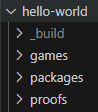
\includegraphics{hello-world.png}
}
\vspace{-1cm}
\end{wrapfigure}

Namely, the hello-world folder contains packages which contain oracle parameters, package state and oracles operating on the oracle state (cf. Section~\ref{sec:packages}), games which contain game parameters and can wire instances of the previously defined packages into a game (cf. Section~\ref{sec:games}). Finally, the proof folder contains one or multiple proofs which contain one more multiple statements to be proven about previously defined games; a proof step is either a \emph{reduction} or a \emph{code equivalence}. See Section~\ref{sec:proofs} for details. Packages have file extension .pkg.ssp, games have file extension .comp.ssp (for \underline{comp}osition), and proofs just have file extension .ssp. Here are three useful commands which you can run in the hello-world folder (or any other project folder):

\begin{description}
\item[cargo run -p ssbee prove:] This command verifies the proof in the folder.
\item[cargo run -p ssbee prove --transcript:] This command verifies the proof in the folder and writes the resulting smt file into hello-world/$\_$build/code$\_$eq, which is usually not needed, but can be interesting if you want to understand what is going on on the SMT level, especially if the SMT solver gives you a counterexample to your proof.
\item[cargo run -p ssbee latex:] This command generates LaTeX code to nicely display the code and games of your project (cf. Section~\ref{sec:latex}) in a PDF. Before doing so, it type-checks the code of packages and games and verifies the reductions, since the command also generates pictures for reductions. This command does not verify code-equivalences.
\end{description}


\subsection{Packages}\label{sec:packages}

\begin{wrapfigure}{R}{0.18\textwidth}
\vspace{-0.75cm}
\scalebox{0.7}{
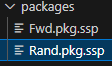
\includegraphics{hello-world-rnd.png}
}
\vspace{-1cm}
\end{wrapfigure}

We explain the structure of a package on the example of the $\M{Rand}$ package in hello-world/packages. Conceptually, this package allows to do a (somewhat) useful operation and a pretty useless operation. The useful operation is that it allows to sample random strings from $\bin^n$ and counts how many random strings it has already sampled. In turn, the (pretty) useless operation takes an integer as input and throws an error whenever that integer is not $1$.

\begin{wrapfigure}{R}{0.615\textwidth}
%\vspace{-0.5cm}
\scalebox{0.37}{
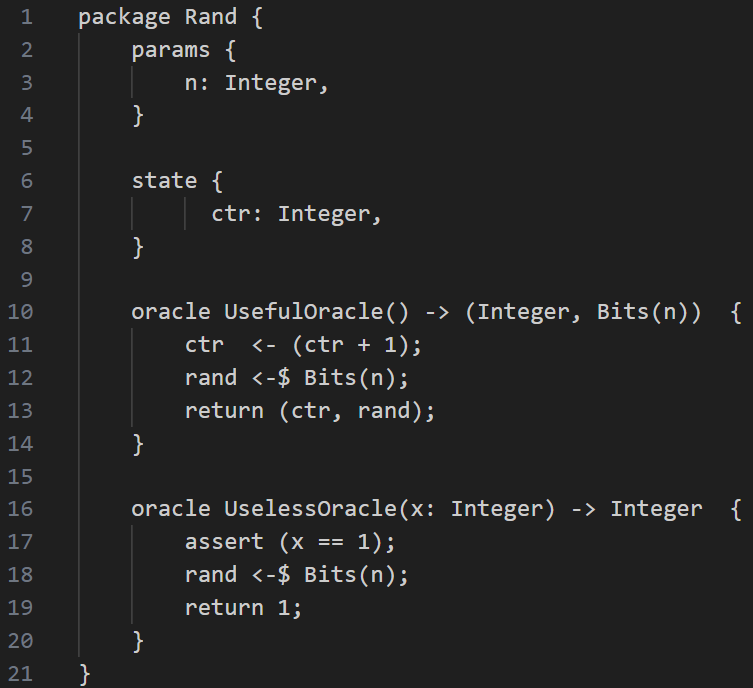
\includegraphics{hello-world-rnd-code.png}
}
\vspace{-1cm}
\end{wrapfigure}

Let's now have a look at the actual implementation of the $\M{Rand}$ package. Concretely, this package has $n$ as a parameter (which is needed to define the set $\bin^n$) and maintains a counter {\tt{ctr}} in its state (which is an integer). The $\O{UsefulOracle}$ can be queried with an empty input, then increments the counter {\tt{ctr}}, samples a random string {\tt{rand}} uniformly from the set $\bin^n$ and returns the pair $({\tt{ctr}},{\tt{rand}})$, i.e., an integer and a string of type Bits(n), our encoding of $\bin^n$. The $\O{UselessOracle}$, in turn, can be queried with any integer $x$. If $x\neq 1$, 

\noindent
the $\O{UselessOracle}$ throws an error (This is the meaning of $\mathbf{assert}$.). Else, it samples a random string {\tt{rand}} uniformly from the set $\bin^n$ (which it does not use and thus is a useless operation) and then returns $1$. See Appendix~\ref{app:code} for a complete description of the SSBee pseudo-code syntax.

Additionally, the packages folder also contains the $\M{Fwd}$ package which also has a $\O{UsefulOracle}$, but its code is different. Namely, when called (with an empty input), $\O{UsefulOracle}$ just forwards the call to another $\O{UsefulOracle}$ oracle (provided by some other package) and returns whatever that call returns.
In turn, $\M{Fwd}$ also has a $\O{UselessOracle}$ with the same code as in the $\M{Rand}$ package, except that it omits the useless additional sampling of {\tt{rand}}.


\subsection{Games}\label{sec:games}
We explain the structure of a game on the examples of the games $\M{SmallComposition}$ and $\M{BigComposition}$ in hello-world/games.


%To turn a package into a package instance, the game specifies
%use the packages and finally one or multiple proof files which specify game instances
%If you run cargo run prove in the hello-world folder, SSBee will verify the proof in hello-world (to be discussed shortly). If you run cargo run latex,

\subsection{Proofs}\label{sec:proofs}


\subsection{Generating LaTeX}\label{sec:latex}


%\begin{abstract}
%Very concrete.
%\end{abstract}

%\tableofcontents

%\section{Introduction}
The paradigm of \emph{reduction-based security}, a.k.a. \emph{provable security}, is the state-of-the-art method of understanding and confirming the security of cryptographic constructions. Concretely, a reduction proof reduces the security of a cryptographic construction (in a model) to the security of the underlying building blocks (in a model). Writing reductions, arguing about their soundness and verifying one's own (or someone else's) proof is relatively easy in some contexts, but it can get out of hand when constructions become complex. Thus, the community develops methods to tame the complexity of security proofs and to increase their precision, including, e.g., \emph{game-hopping}~\cite{EPRINT:Shoup04}, \emph{code-based} arguments~\cite{EC:BelRog06} as well as composition frameworks such as Universal Composability~\cite{FOCS:Canetti01} and Constructive Cryptography~\cite{FC:Maurer10}.

Nevertheless, studying protocols such as Transport Layer Security (TLS~\cite{TLS13})
and Messaging Layer Security (MLS~\cite{MLS}) \emph{as they are} 
%(without simplifications and abstractions) 
remains difficult, since their description exceeds 100 pages which makes the protocols unwieldy for analysis without simplifications. Similarly, other real-life systems tend to combine multiple cryptographic components in complex dependencies,
see, e.g., remote attestation mechanisms~\cite{https://arxiv.org/pdf/2102.08804.pdf,https://en.wikipedia.org/wiki/Trusted_Computing}, ... or ... .

The challenge when analyzing complex protocols is three-fold:
\begin{description}
\item[(1) Large protocol description.] The description of a protocol itself exceeds the bounds of a research article.
\item[(2) Consistent code-base.] Parts of the protocols are referred to multiple times in an analysis and maintaining a consistent version of a complex protocol throughout the analysis is difficult.
\item[(3) Large reduction description.] Describing reductions entirely exceeds the bounds of a research article since they typically emulate most of the protocol.
\item[(4) Verifying reductions.] Verifying reductions is tremendously challenging due to the complexity of both the reduction and the protocol.
\end{description}

Item (1) and (2) can be mitigated by describing the protocol
modularly and maintaining a single code-base for the protocol
whose components are imported into the analysis whenever needed.
However, typically, an important component of protocol analysis 
is to re-write a protocol (and the game around it) in a 
functionally equivalent way that is easier
to analyze (cf. Bellare-Rogaway code-based
game playing~\cite{EC:BelRog06}).
% or matches the shape of the reduction---in a way, 
Similarly, writing a reduction typically includes re-writing the protocol 
except for a small component which, instead of being locally evaluated, 
is forwarded to an oracle by the reduction. Establishing (perfect) soundness of 
a reduction is then, again, a proof of functional equivalence\footnote{Large 
real-life protocols typically only employ straightline reductions. The 
above proof outline does not apply to, e.g., rewinding, but it would 
allow, say, programming a random oracle. Also note that proving functional equivalence 
up to statistical difference can be avoided by first making a game-hop
bounded by a statistical difference.}. Thus, protocol analysis regularly
requires us to prove functional equivalence between different protocol descriptions,
reductions and games.
% Thus, we need to prove functional equivalence between 
%large protocol components. Similarly, for reductions, we need to
%prove that a reduction emulates a high-level game correctly while
%interacting with a low-level game that it tries to win. These proofs, too,
%are functional equivalence proofs for complex objects.

\paragraph{Verifying Code-Equivalence.}
Indeed, the core component of the pioneering formal
verification tools CertiCrypt~\cite{X} and EasyCrypt~\cite{X} for 
cryptographic reductions are functional equivalence proofs. Since functional 
equivalence is coNP-complete\footnote{An input $x$ such that 
$f(x)\neq g(x)$ shows that $f$ and $g$ are not code-equivalent.} and 
for randomized programs even higher up the polynomial hierarchy\footnote{We need to prove that the \emph{distributions} $f(x)$ and $g(x)$ are identical.}, 
CertiCrypt and EasyCrypt do not verify functional equivalences automatically.
Instead, functional equivalence is proven interactively: The user writes
a proof consisting of small, detailed steps which the tool verifies.
%but rather require the user to write a proof of functional equivalence
%consisting of small, detailed steps. 
As an example, the EasyCrypt formalization
of a proof for Yao's garbled circuits~\cite{X} shows that after polynomially many game-hops, a simulated garbling can be computed without knowing the input and while only knowing the output of the circuit evaluation, thus establishing the desired goal that a garbled circuit does not leak any information beyond its output value (which can
always be trivially derived, see~\cite{X} for more discussion). This code equivalence proof between two versions of the garbling, one with and one without
knowing the input, consists of ... lines of code in EasyCrypt (~\cite[page x]{X}).
%EasyCrypt,
% thus, indeed enables us to verify complex code equivalence proofs.

In turn, in the pen-and-paper proof of Yao's garbled circuits by Lindell and Pinkas, the analogous conceptual argument consists of 10 lines of text (\cite[page 23]{x}, which is the ePrint version of~\cite{X}); and in the pen-and-paper proof of Yao's garbling scheme by Bellare, Hoang and Rogaway, ...(\cite[page ..]{X}). Both code equivalence proofs consists of a conceptual high-level argument about distributions of keys, while the EasyCrypt analysis (a) additionally makes explicit which randomness for key sampling in one game corresponds to randomness for key sampling in the other game and (b) ... .

\paragraph{Proving Code-Equivalence Proofs.}
The aforementioned example of Yao's garbling scheme illustrates that current
computer-verified proofs provide higher assurance, but do not reduce the
workload in analyzing a complex protocol, but instead
%
%don't necessarily
%help us address the problem of navigating too complex protocols,
%since even apparently simple steps 
require significant additional work
beyond the amount of detail typically worked out in pen-and-paper proofs. 

Thus, a natural question is whether we can not only \emph{verify} but
perhaps also \emph{automatically} prove code equivalences. As mentioned
before, program equivalence is (at least) an NP-complete complete problem.
However, SMT-solvers such as Z3~\cite{X} and CVC4~\cite{X} excel in 
solving structured, practical instances of NP-complete problems, so it
seems worth investigating whether program equivalence as it emerges in
the context of cryptographic reductions could be solvable by an off-the-shelf
SMT-solver. %Jumping ahead, in this article, we give evidence that proving
%code-equivalences can be significantly automatized, see Section~\ref{X}.

\paragraph{Managing code and incremental changes.}
Returning to item (1)-(3) above, proofs for large protocols require, in fact,
a large amount of code which needs to be maintained consistently: In terms of
basic objects, there are the protocol, the game describing its security as well
 as the games describing the underlying assumptions. Furthermore, a game-hopping
proof typically requires describing hybrid games, each of them with an inlined
version of the protocol where parts of the component might have been replaced
by idealized versions, e.g., a truly random function instead of a pseudorandom function (PRF). Additionally, each game hop comes with the description of a reduction.

The result of (successful) proof development is an article where all of the
above are consistent and where equivalent descriptions of a game have
been proven equivalent and reductions have been proven to be sound.
However, the \emph{development phase} proceeds via many stages where
we prove statements about games which later turn out not useful or
which have small errors and inconsistencies that we correct later.

When considering code modifications to correct errors, these changes do not
propagate automatically---in fact, we need to backtrack which pieces
of code are affected, which code-equivalence statements fail now etc..
Under the assumption that off-the-shelf SMT solvers can verify
code-equivalence statements and under the assumption that we have
made all reductions explicit in some formal language, we can, at 
any point of time, ask an SMT solver to (re-)prove all statements and thus see which
statements are affected by a modification. However, since most proofs
of large real-life protocols consists of many game-hops, we usually only
specify the hybrid games in pseudocode, but not the reductions, and
writing the reductions seems undesirable overhead, even if in return, we
get the (potential) benefit of automated verification and continuous 
integration.

\paragraph{State-separating proofs.}
An exception to the practice of incomplete game and reduction descriptions for
real-life protocol analysis is the state-separating proof methodology (SSP),
introduced by Brzuska, Delignat-Lavaud, Fournet, Kohbrok and Kohlweiss (BDFKK~\cite{X}). SSPs suggest to write code of games and protocols modularly in (stateful) packages which call one another via oracles but cannot access each others state other than
via oracle calls (whence their name). 

Modular code writing and code re-use has already been suggested in Bellare and Rogaway's original work~\cite{X} (TODO: check that this is true.) and been practiced, e.g., by BHR~\cite{X}, where TODO: example.
The SSP methodology (cf.~\cite{X,Y,Z}) develops this idea systematically further and ties it in closely with \emph{compositional} aspects. Concretely, an SSP package typically consists of code and state that is \emph{shared} between multiple cryptographic primitives and/or their games. Subsequently, we can specify reductions precisely in pseudo-code \emph{without} writing any new code, simply by re-using existing packages and composing them into a call-graph. Indeed, all existing works on SSPs make use of this feature~\cite{blankedcite}.

A downside to defining games via call-graphs of packages is a fragmented
description of games: To fully understand a game, we need to consider the
call-graph at the same time as the code of its building blocks, leading
to challenges in the presentation (cf.~\cite{ACNS:BEP24} for a discussion).
Moreover, the code of a single package is now re-used by many different games, 
so that changing the code of a package affects many definitions and proof 
steps at the same time.

Thus, SSPs would benefit from automated sanity checks such as oracle signatures
(the caller of an oracle includes the arguments that the callee expects) as
well as the aforementioned continuous integration approach.
Additionally, SSPs come with a high level of precision and
that is suitable for formalization. Hence, all-in-all, SSPs are an ideal
candidate to provide a tool-based development process
that is \emph{less} work than its pen-and-paper counterpart
and at the same time leads to computer-verified proofs.

%, automatization and,
%all in all, for using tools that not only \emph{verify}
%proofs, but actually support a tool-based proof development process
%that \emph{less} work than its pen-and-paper counterpart.

\subsection{Our contribution.} After a major development effort,
we present SSBee, a novel tool to support SSP-style proofs. 
In SSBee, the user can specify packages and call graphs in a 
pseudocode-style (see Section~\ref{X} for details), while SSBee
checks the consistency of the resulting composition. Subsequently,
the use can specify sequences of games, where each game-hop consists
either of a code-equivalence step or a reduction to an underlying
assumption. Since we consider SSPs, the latter merely consists in
specifying a sub-graph (and verification is not a major challenge).
As for EasyCrypt, the main challenge are code equivalence proofs.
We elaborate on code equivalence proofs shortly, but first would
like to emphasize that the use of SSPs \emph{reduces} the number
of code-equivalence proofs, since a suitable modularization of a game
typically only requires one code-equivalence proof in the beginning
and one code-equivalence proof in the end of a proof sequence.
See Section~\ref{X} and Kohbrok~\cite{Kohbrok:thesis} for a details.

\paragraph{Code-Equivalence Proofs}






present SSBee, a tool that does all the things
we said above would be great. It maintains code for SSPs, checks code-equivalences
semi-automatically and provides continuous integration support.

On a technical level, we support all sorts of things in code, including for loops
and poly many hybrids.

On a user interface level, we can export to LaTeX and proof viewer, both graphs and packages which might make it easy to communicate what one proved in a paper but
deferring the (consistent) things to the prover.


%to support the development
%of proofs in SSP-style.


% as well as (partial) automatization of code-equivalence
%proofs via SMT-solvers.




%other works, where to go from here
%---in fact, they have been formalized both in EasyCrypt~\cite{X}
%and Coq~\cite{X}.

%The code-reuse allows to define new games and reductions precisely, and
%verifying cuts in graphs 






TODO:
- Mention that SSPs reduce code-equivalences.
- Mention that EasyCrypt does distributions, nut 
- using SMT-solver for hybrid indices, um zu schauen dass sie bijektiv





=== stopped here, somehow, the flow broke ===

{\color{gray} Not yet integrated into the flow




 
Firstly, one needs to maintain a comprehensive, consistent description of
a protocol that has an extremely 



While these aforementioned protocols have been actively studied~\cite{X}, a comprehensive analysis without 


Therefore, TLS 1.3 as it is has only been studied via formal methods. Concretely, the celebrated miTLS work ...~\cite{X} ... something about code-base... However, $F^*$-based verification alone does not enable obtaining reductions to the underlying assumptions and was thus complemented with paper-based reductions of the cryptographic core.

For TLS 1.3, the cryptographic core or \emph{key schedule} has recently been analyzed (without simplifications) by Brzuska, Delignat-Lavaud, Egger, Fournet, Kohbrok, and Kohlweiss (BDEFKK~\cite{X}).
%, providing an interface which aligns with the $F^\star$-based analysis of ... . 
Towards this goal, Brzuska, Delignat-Lavaud, Fournet, Kohbrok, and Kohlweiss (BDFKK~\cite{X}) had previously developed \emph{state-separating proofs (SSP)}, a definitional style and proof methodology that allows to specify games via graphs of stateful code packages and enables precise reduction (and their verification) by
specifying a ``cut'' in the graph of a game (see Section~\ref{X} for details on SSPs).

Subsequently to BDFKK and BDEFKK, in his thesis, Egger~\cite{X} reduces the security of TLS 1.3 as a key exchange protocol to the security of the TLS 1.3 key schedule. Egger's proof covers all ``TLS-like'' protocols. The need to abstract TLS 1.3 into the class of TLS-like protocols, again, resides in the fact that TLS 1.3 has a long description which is unwieldy for a pen-and-paper proof. Moreover, his proof consists, essentially, of 5 code equivalence proofs which Egger proves via complicated and detailed code equivalence proofs. Such complicated detailed proofs are necessary to obtain a reasoneable level of assurance, but they are hard and tedious work to establish statements that, on a high-level are rather simple.

Therefore, it would be appealing to delegate these code equivalence proofs to
a designated tool. Handling the code equivalence proofs by a tool would also
allow to handle larger code than we are able to manipulate by hand, such as the
code of the entire TLS 1.3 protocol.

In addition to making certain results feasible at all, a designated tool could 
also simplify the work on SSP-based proofs altogether, such as maintain a consistent
code base and automatically verify that components are indeed compatible.
Moreover, it could, in general, relieve researchers from needing to prove
code equivalence proofs, whether they are easy or not. For example, Brzuska
and Oechsner (BO~\cite{X}) in their SSP-style proof of Yao's garbling scheme,
use a code-equivalence proof to prove that so-called ``semantic switch'', where
wires are associated with the role being ``active'' or ``inactive'' rather than
being a $0$-key or a $1$-key. BO also require two additional code equivalence proofs
to reduce their SSP-style IND-CPA notion to standard IND-CPA and to show that their
SSP-style garbling security notion implies standard semantic security of garbling schemes. The entire article would become significantly simpler if these equivalence
proofs could be discharched to a tool.





%Issue: I actually don't know what miTLS proves and whether it is enough to say that it does what we want or not. I should probably study the interface --- and maybe, here, it is worth to talk to Konrad, Hakon, Antoine and Markulf...

\iffalse
=== OLD ===

Designing cryptographic constructions, reductions, proving their soundness and verifying the correctness of one's proofs is, at times, a difficult endeavour, because constructions can be complex (e.g., TLS 1.3~\cite{X}), reductions can be complex (even for simple constructions such as the Goldreich-Levin hardcore bit~\cite{X}), proving the soundness of a reduction can be intricate and subtle even for simple reductions (e.g., the random embedding reduction in Yao's weak-to-strong one-way function amplification), and verifying the overall proof is typically difficult because we tend to use significant amount of conceptual high-level reasoning which one needs to reproduce when verifying the proof (e.g., understanding why/how the orginal Lindell-Pinkas reduction proof for Yao's garbling scheme~\cite{X} uses an additionally provided encryption oracle of the underlying security notion for symmetric encryption and why this suffices to conduct a hybrid argument over the circuit in topological order).

\subsection{Supporting protocol and proof development and verification}
We categorize research on supporting these different stages of designing a protocol and developing and verifying the associated reduction proofs into the following four (overlapping) categories (1) attack-finding, (2) composition, (3) proof-writing styles and (4) formal verification and now briefly review each.

{\color{blue}
\paragraph{Attack-finding.} Tamarin (+ application to TLS, MLS), and why do I call this attack-finding (one can also call this automated proving, but should rememember that the adversary can only do a certain kind of operation). Briefly mention that the gap between the symbolic approach and the reduction-based approach can, in principle be bridged (computational soundness, Abadi-Rogaway), and that there is some research in this direction of doing this (still today).

\paragraph{Composition.} UC, random systems, constructive crypto, SSPs}

\paragraph{Proof-writing styles.}
%Cryptographic proof-writing style has significantly evolved throughout the
%development of the field. In 2004, 
Shoup explicates \emph{game-hopping} in order to advertise its use as a tool for taming complexity in security proofs. 
%In 2005,
Bellare and Rogaway introduce and advertise a \emph{code-based} variant of
game-hopping, treating code as semi-formal objects. 
%20 years later, 
%most reduction proofs in the field are structured into sequences of games, and a
%significant portion of them is also \emph{code-based}. 
The aforementioned state-separating proofs can be viewed as a refinement of code-based game-hopping which allow to construct reductions as cuts in graphs, so that proving/verifying the soundness of a reduction boils down to observing equality call graphs consisting of code-packages.

\paragraph{Formal verification of reductions.} 
%While attack-finding tools such as Tamarin also establish the absence of attacks in a symbolic model with idealized cryptographic primitives, Tamarin cannot help with verifying reduction proofs, as mentioned above. 
Interactive theorem provers such as Coq~\cite{X} allow one to computer-verify a
proof as long as it is written as a sufficient level of precision of detail.
The pseudo-code-based approach by Bellare and Rogaway explicates a proof style which is suitable for actual formalization, since all games and reductions are explicitly written in pseudo-code. Inspired by Bellare and Rogaway, in a pioneering work, X, Y and Z developed CertiCrypt~\cite{X}, the first approach for verifying cryptographic reductions, followed by A, B and C developing EasyCypt~\cite{X} as a first tool \emph{independent} of Coq. One of the important technical contributions of CertiCrypt/EasyCrypt is a method for proving the \emph{soundness} of a reduction which requires proving that two stateful, randomized, interactive programs have identical input-output behaviour. While research articles usually use high-level conceptual reasoning for this purpose, computers need more detailed and precise arguments, and a priori, it is unclear how to translate the high-level reasoning into a sufficiently formal and detailed language. We provide more technical details on how to successfully resolve this issue in Section~\ref{X}.

\subsection{Halevi's vision and beyond}
Halevi~\cite{X} joins Shoup, Bellare and Rogaway in the quest for
high-quality proofs by presenting a dream-vision of computer-assisted 
cryptographic proving. Namely, Halevi perceives designing cryptographic 
schemes and reductions as the \emph{creative} part of cryptographic research, 
while he perceives checking the soundness of reductions as \emph{mundane}. 
Thus, Halevi hopes for assistance in the development of proofs, relieving 
the researchers of work perceived as tedious: Checking the soundness 
of reductions shall be carried out by computers \emph{automatically}.

Unfortunately, computer-verification requires a detailed presentation of a 
proof argument in order to verify it and thus, while the current state-of-the-art
indeed allows to check the soundness of a reduction, it is far from automatic.
Instead, the user needs to provided a detailed proof of the soundness of the
reduction which is then verified---and thus, currently, using computer-verification
to check reduction proofs is very far from reducing work, let alone relieving
cryptographers of the work required for checking the soundness of a reduction.

A very useful question, closely related to Halevi's vision, is how
computer-assistance can generally relieve cryptographers from work perceived 
as tedious or difficult. %For example, Tamarin~\cite{X} checks the high-level
%logic of complex protocols.
As a simple example, maintaining pseudocode for games and reductions in a single 
code-base prevents inconsistency across a research article where the same code
is used in multiple places. Similarly, certain sanity checks on a reduction
are quite easy to carry out such as whether the reduction correctly accesses the
oracles of the underlying assumption. Moreover, while in general, proving the soundness of a reduction requires hard-to-formalize conceptual reasoning, the aforementioned graph-based SSP reductions merely require checking graph equality,
which is tedious for a human when the graphs are large, but easy for a computer in the case of the layered directed acyclic graphs (DAGs) used in SSPs. {\color{blue} Not sure that this is true, but it sounds nice. Somewhere, there should be an SSP intro, not sure yet where. In the text below, please assume that SSPs have been properly introduced---but I still need to find a place for them, maybe discuss proof viewer.}
\fi

\subsection{Our Contribution}
We develop \emph{SSBee}, an independent tool which allows to specify and maintain
SSP packages in pseudocode, compose them into games as well as write and verify
SSP-based game-hopping proofs. Additionally, SSBee visulizes all games and proofs in the SSP proof viewer~\cite{X} and exports pseudocode to LaTeX in order to achieve consistency between the code-base maintained by SSBee and a research article
presenting the main results. As a first case study, we implement and verify the SSP-based reduction proof for Yao's garbling scheme by Brzuska and Oechsner~\cite{X}. Moreover, since the goal of SSBee is to support the \emph{proof development} rather than merely check existing proofs, we also extend the work by Brzuska and Oechsner to compose Yao's garbling scheme with a random oblivious transfer protocol (OT) into a secure 2-party computation protocol with semi-honest security. While this result has already been proven by ...~\cite{X}, it is an interesting and meaningful extension of the original case-study by Brzuska and Oechsner since it formalizes and proves security of a secure 2-party computation protocol in SSPs for the first time. Moreover, it informs us about a natural workflow which a user might adopt.

\subsection{Workflow}
In a natural workflow, the users sketch SSP graphs and the sequences of game-hops
on paper. Here, each package has an intended behaviour that has not been fully
specified or formalized yet but that the user finds convincing. Subsequently, when
the user wants to verify their conceptual ideal, they specify the behaviour of packages
as SSBee pseudocode and construct / compose their packages into the games previously sketched on paper. In this stage, code and package compositions mature jointly, and SSBee checks the interfaces of packages to one another. Next, the user specifies all games which occur in the game hops using the previously defined packages.
SSBee immediately verifies all graph-based game-hops in this step and thus verifies that the reductions have the correct interface. Finally, the user specifies all \emph{perfect equivalence} steps, which, in most cases, are verified automatically by SSBee, using an SMT-solver beneath. In conceptually involved cases, users need to provide some \emph{core} argument from which SSBee completes the equivalence proof automatically.
%These are game-hops where one game is replaced by another whose behaviour is perfectly equivalent. While SSPs typically allow to reduce the number of perfect equivalence steps, a few still need to be carried out and they are, typically, terribly tedious and hard to carry out on paper. These steps are, indeed, conceptually similar to checking the soundness of reductions in the traditional style. While SSPs do not require carrying out such steps for each reductions, a few still remain and one needs to do them. This step is where SSBee comes close to realizing Halevi's vision. In conceptually involved cases, users need to provide some \emph{core} argument from which SSBee completes the equivalence proof automatically. Moreover, in easier cases, SSBee  generates and verifies equivalence proofs entirely automatically. Details follow.

\section{Technical Approach and Scope}
\subsection{Induction over oracle calls}
When arguing in research articles, we typically compare the behaviour of
two cryptographic games \emph{directly}, discussing how the state in each
of the games evolves in relation to each other and why, e.g., both games
provide the same restrictions on their decryption oracle (cf. page ..in~\cite{X}).
%, e.g., by arguing that swapping two
%lines of code does not affect behaviour if the two lines operate on independent 
%state.
In order to formalize this argument, we need to show that on \emph{all} sequences of inputs, the oracles of the two games provide the same output. A clean way of formalizing this argument is via \emph{induction} over all sequences of oracle calls. We first define a relation between the state of the two games, then show that the relation holds in the beginning of the game and, additionally, that if the relation holds before an oracle call, then the relation holds also after the oracle call and the oracles of both games indeed return the same output. If the two games are very similar, the state relation can be simply equality.

Moreover, when the games are randomized, we need to argue about \emph{distributions}
of outputs rather than equality of outputs. A clean way to extend the above induction-based approach to randomized programs is by providing a bijection $f$ between
the random strings consumed by the oracle of the two games which leads to the
same output.

This \emph{invariant}-based approach with randomness mapping has been developed in the context of EasyCrypt {(\color{blue} True ?? Probably older...)} and we also adopt it in SSBee.

\subsection{Automatization}
Given a state relation and a randomness mapping, EasyCrypt additionally requires
proving that the state relation is an invariant {\color{blue} I don't like writing this.}. In turn, SSBee seeks to avoid that the user needs to do these additional proofs. Therefore, SSBee translates the pseudo-code based statements into SMTlib statements. SMTlib~\cite{X} is an interfacing language for SMT solvers and currently supported by Z3~\cite{X} and CVC5~\cite{X}. The SMT solver is tasked with showing that (i) the randomness mapping is valid (i.e., is a bijection), that (ii) the state relation is an invariant and (iii) if the state relation and the randomness mapping holds, then equal inputs lead to equal outputs.

In general, (iii) is an NP-complete problem. However, it turns out that for the instances we consider in our case studies, CVC5 are able to prove (iii) within a few seconds. An exception is the difficult proof step in Yao's garbling scheme which performs a switch from bit semantics to active/inactive semantics. Here, we need to specify an additional lemma, and CVC5 needs 30 seconds to prove (iii).

\subsection{Multi-instance packages, \textbf{for} loops and hybrid arguments}
SSBee supports multi-instance packages, \textbf{for} loops as well as hybrid arguments over polynomially many hybrids. Multi-instance games allow complex
compositions of a polynomial number of packages or number of compositions of
a priori unknown number of packages.

In the case of \textbf{for} loops, the user needs to specify additional loop invariants (EasyCrypt does this also).

For polynomially many hybrids, the user needs to specify ... as outlined in Appendix B of ... in the hybrid argument recipe.




\subsection{Limitations and future work}
no statistical game-hops (--> combine with easycrypt)
no verification of code in Coq (--> combine with SSProve somehow?)
SSP-style-only (--> inherit limitations of SSPs, no rewinding for now)





==== OLD OLD OLD ===



Halevi~\cite{X} joins Shoup, Bellare and Rogaway in the hope for improved quality of proofs by presenting his dream-vision of computer-assisted cryptographic proving and, implicitly, also pointing to a cause of what he calls a \emph{crisis of rigour}.
Namely, Halevi perceives designing cryptograhic schemes and reductions as \emph{creative} part of cryptographic research, while he perceives checking the soundness
of reductions as \emph{mundane}. Thus, Halevi hopes for assistance in the development
of proofs, relieving the researchers of work which they perceive as tedious: Checking the soundness of reductions shall be carried out by \emph{computers} automatically.

In a pioneering work, ... indeed enabled the checking of reductions by computers. However, unlike imagined by Halevi, checking the soundness of reductions in EasyCrypt is not \emph{automatic}. First, all games and reductions need to be formalized in the (very appealing) language of EasyCrypt. Subsequently, the equivalence between two adjacent game or the equivalence between a high-level game on the one hand and, on the other hand, a reduction composed with a game specifying an assumption, these equivalences need to be proven by first formulating an invariant, then proving in the EasyCrypt proof language that the invariant is an invariant and showing functional equivalence of two games by induction over the oracle calls\footnote{Cryptos will not understand this, needs to improve.}. EasyCrypt is a masterpiece of formal verification software and able to argue about complex programs using for-loops and also able to establish proofs of statistical closeness, both of which are notoriously difficult problems in formal verification. However, while being an extremely impressive formal verification tool, EasyCrypt is not widely used across the cryptographic community, because it does not address Halevi's vision: Using EasyCrypt, the work invested into proving equivalences / soundness of reductions is not decreased, but rather increased. EasyCrypt is expert in checking the correctness of a proof, but EasyCrypt is not a helpful tool for developing new results in cryptography.

Before accusing EasyCrpyt of not being sufficiently ambitious, we should consider criticizing Halevi for posing an overly naive vision. Proving equivalence between two (poly-time) programs is, in general, coNP-complete, and proving equivalence of two \emph{stateful}, \emph{randomized} (poly-time) programs is in the ... level of the polynomial hierarchy. Of course, SAT-solvers are apt at dealing with structured real-life instances (cf.~\cite{X,Y,Z} and references therein) of NP-complete problems, but typically do not target the ... of the polynomial hierarchy, and rarely aim at proving equivalence of randomized programs, let alone argue \emph{inductively} about interactive \emph{stateful} programs and their behaviour.

Given this dire state of affairs, a \emph{general} push-button tool for proving soundness of cryptographic reductions seems unrealistic based on the current state-of-the-art in automated solvers. However, given a state-relation and a \emph{randomness mapping}\footnote{Cryptos will not know what this is.}, proving that the state-relation is an invariant if the randomness mapping holds is ``only'' coNP-complete, and so is proving that the output of the two oracles is identical if the state-relation and the randomness mapping holds. Thus, with slightly more input from the working cryptographer, the proof might move into the range of what an automated solver is able to show, and in many cases, randomness mapping and state relation are completely trivial and can be generated automatically.

Still, computer-verification according to the above strategy requires fully writing a reduction in pseudo-code rather than describing it conceptually on a high-level, e.g., \emph{the reduction behaves like the game except for calling its \O{EVAL} oracle instead of evaluating the PRF} would need
to be replaced by a large piece of pseudo-code which consists of the full game description where the calls to the PRF are replaced by \O{EVAL} oracle calls.
Writing the reduction's pseudo-code is not infeasible given that one already
wrote the code for the game. However, we might still not be able to argue that 
the entire formalization is less tedious than carrying out the soundness proof manually.

Thus, the key question is where the above approach \emph{supports} the cryptographer
in their proof development and \emph{eases} their proof development rather than adding more work and steps to it\footnote{Again, the extra work comes with extra guarantees, and those might be worth it, but will cryptographer be willing to go this extra mile?}.

\paragraph{Our contribution.} As we show in this article, proof development is \emph{eased} via the above strategy when applied to proofs in the state-separating proofs framework (SSP~\cite{X}). [..]

\iffalse
\clearpage
OLD OLD OLD



Halevi's dream-vision of computer-aided reduction proofs in cryptography~\cite{Halevi} hopes that one day, while creativity is still reserved for humans, algorithms will be in charge of tedious steps which confirm the soundness of a reduction and only use standard techniques. An important, somewhat orthogonal, success on the path for computer-aided cryptography is that computer-aided \emph{attack-finding} has established itself firmly as a standard tool for protocol development. Most importantly, Tamarin~\cite{X} has been used to improve ...~\cite{X}, ...~\cite{X} and ...~\cite{X}, and, in particular, is used across the community also without involving an author of the original tool, see, e.g.~\cite{X}. However, computer-aided \emph{reduction proofs} have not yet joined the quest to inform protocol design quickly. In fact, to date, reduction proofs for large protocols such as TLS and MLS have not been computer-verified, let alone been helped by algorithms, and indeed, we do not yet have the tools to do so.

One core reason is that invoking the help of a computer requires formalizing one's proofs at a level of detail which is unusual for standard mathematical practice, including cryptography. For example, one might describe two security games and a construction in English, then describe a reduction in English and prove its soundness by arguing about difficult key points. In their celebrated foundational work, Bellare and Rogaway~\cite{X} encouraged the community to use \emph{code} to describe their reductions, games and game-hops and demonstrated how code-based argument allow us to obtain a neat proof for ... . This leap towards more precision enabled ... ... and ...~\cite{X} to develop the pioneer tool EasyCrypt for verifying cryptographic reductions. EasyCrypt has been used to verify ... ,... and ... as well as a proof of Yao's garbling scheme~\cite{X} as one of its largest case studies. Simultaneously, Bellare-Rogaway-style game-hopping has become an established technique in our community. Similarly, the composition frameworks Universal Composability (UC~\cite{X}) or Constructive Cryptography (CC~\cite{X}) have a large and growing user base who write their reduction proofs in these frameworks (cf. ... and references therein). This suggests that our community is willing to invest time and effort into writing clearer proofs, but the overhead currently required by EasyCrypt is still considered prohibitive. 

A recent arrival to the family of composition frameworks are \emph{state-separating proofs} (SSPs~\cite{X}) where the first large case studies have been published over the past 2 years. Concretely, SSPs have been used to provide reductions for the key derivations in both TLS~\cite{X} and MLS~\cite{X} and, most recently, to give a novel security reduction for Yao's garbling scheme~\cite{X}, demonstrating the potential feasibility to use SSPs also for secure multi-party computation.

Similarly to Bellare and Rogaway's code-based game-playing, SSPs, a refinement of Bellare-Rogaway, are formalization-friendly and have since been formalized in Coq~\cite{X} as well as in EasyCrypt~\cite{X}. In fact, SSPs have become a useful manual prototyping step for developing proofs in EasyCrypt [Dupressoir-Oechsner, personal communication :-)]. What is missing, still, however, is a formal verification tool which \emph{helps} cryptographers in the \emph{development} and \emph{execution} of their proofs and not only in the verification.

\paragraph{Our contribution.} In this paper, we provide such a tool for SSPs: SSPVerif. 
%SSPs have shown to be useful to carrying out proofs for large real-life protocols~\cite{X,Y} and thus, focusing on SSPs is a useful scope. 
We built SSPVerif, because in our development of handwritten SSP proofs for large protocols, we struggled (a) with the \emph{maintainance} of a \emph{large code-base}, (b) with verifying the \emph{consistency} of the code-base and last, but not least, (c) with carrying out code-equivalence proofs. The latter cover ... pages of the security analysis of TLS 1.3~\cite{X} and ... out of ... in the reduction proof for Yao's garbling scheme~\cite{X}. They have been completely avoided in the security reduction for MLS by the use of modular assumptions and modular top-level target security definitions~\cite{X}.

SSPVerif addresses (a) and (b) by checking consistency of packages and their compositions as well as exporting to LaTeX for a consistent research paper. For (c), code-equivalence proofs are discharged to an SMT-solver, either CVC4~\cite{X} or Z3~\cite{X}. Our case studies demonstrate that CVC4 and Z3 are, indeed, sufficiently powerful to prove typical code-equivalences with no to little manual support. 

\paragraph{Case studies}
Yao (compare with EasyCrypt), NPRF

\paragraph{Features}
for loops, multi-instance, type system

\paragraph{Limitations and future work}
SSPVerif is automatized but special-case, EasyCrypt/SSProve is general, but not automatized. Can we use SSPVerif for prototyping of invariants for EasyCrypt/SSProve? Can we use EasyCrypt to prove assumptions used in our SSP proofs. Integration with proof viewer.





\iffalse
It is no co-incidence that EasyCrypt~\cite{X}, the pioneer tool in verifying cryptographic reduction proofs, is based on Bellare and Rogaway's code-based game-hopping~\cite{X}. Namely, Bellare and Rogaway specified 



While computer-aided attack-finding has become a standard tool in protocol development


In a celebrated breakthrough, Abadi and Rogaway~\cite{X} showed that 









==== EVEN OLDER ====


Since Halevi~\cite{X} declared a \emph{crisis of rigour} for reduction proofs in cryptography
and called for tool support to leave the \emph{interesting} steps to the creative cryptographer
and the \emph{mundane} steps to a powerful automated tool, significant progress has been made
towards this vision. In particular, Dupressoir and some others~\cite{X} formalized the Bellare-Rogaway
code-based game-playing~\cite{X} approach in EasyCrypt which now allows to verify code transformations
and reduction-based game hops. 

EasyCrypt does not take care of mundane steps fully automatically, as in Halevi's vision, but rather is semi-automated
and usually requires cryptographers to write pre-conditions and post-conditions (or simply a single invariant) and prove
that if the pre-condition was satisfied before an oracle call, then the post-condition is satsified.
The reason that the SMT solver underlying EasyCrypt cannot prove code equivalence without additional
help is that conceptual high-level reasoning is not part of the solver. The present paper does not
change this state of affairs, but instead increases \emph{modularity} of the EasyCrypt technique.

Concretely, we present SSPVerif, a new verification tool for cryptographic game-hopping proofs which
is based on \emph{state-separating proofs} (SSPs), a recent, modular technique for game-hopping in pen-and-paper
proofs. SSPs structure code of cryptographic protocols and security game as stateful pieces of code
called \emph{packages} which can call one another, but otherwise do not share state. Since package
composition is associative, one can simplify complex game-hops by ``pushing code into the adversary''
(cf. Section~\ref{X}).

SSP-style techniques have already been formalized in EasyCrypt~\cite{X}, but since package are not
native in EasyCrypt, the implementation does not provide SSP-specific support and, in particular,
the SSP-style workflow. SSPs have also been formalized in SSProve~\cite{X}, a Coq-based tool specially
developed for SSPs, but no large examples have been shown in SSProve. In turn, SSPVerif has been developed
to especially support the workflow of the working SSP cryptographer.

As an example, we use Yao's garbled circuits: much larger than what is known in SSProve; Yao has already 
been done on EasyCrypt, so great test case.
\fi
\fi
}
%\section{State-Separating Proofs}
adopt Yao intro?
%\section{SSBee}
\subsection{Pseudo-code}
We already saw an example of SSBee pseudocode in Section~\ref{sec:ssp} and now discuss the features and limitations of SSBee pseudocode more comprehensively.
In terms of basic operations, SSBee pseudocode supports assignment to state variables and temporary variables (whose value will be forgotten after the oracle call), creating and parsing tuples, sampling uniformly from a set, and evaluation of unspecified function as well as oracle calls. State variables can be individual values or tables. Pseudo-code can contain a special $\mathbf{assert}\mathsf{ cond}$ command which aborts the oracle run if condition $\mathsf{cond}$ is violated. Moreover, SSBee supports if-then-else branching as well as for loops.

\paragraph{Type system.}
SSBee operates on typed symbols, e.g., symbols can be integers (Int),
Booleans (Bool), bitstrings of length n (Bits(n)), tuples of values,
tables etc.. Moreover, the user can specify additional types. For 
every type $\mathsf{type}$, the operation $\mathsf{Maybe}\;\mathsf{type}$
creates a larger type which contains $\mathsf{type}$, but a value
might also be $\mathsf{none}$.

Maybe types are particularly useful for tables. Concretely, at each position, a table might either have a value or be unassigned. Thus, when accessing a table at a position, it is unclear whether it is of the type of values that the table typically contains or of type $\mathsf{none}$. Therefore, a value $v\leftarrow T[i]$ is considered to be of $\mathsf{Maybe}\;\mathsf{type}$, and to turn $v$ into $\mathsf{type}$, we ... which we can only apply if we are guaranteed that $v\leftarrow T[i]$ is not 
equal to $\mathsf{none}$.

\paragraph{Limitations of SSBee pseudocode.}
Sampling from arbitrary distributions needs to be modeled by sampling uniformly from
a set and applying a function to the result. Since SSBee pseudocode is symbolic, it
does not have a concept of length for bitstrings. As a result, in the IND-CPA encryption example, the oracle accepts messages of a \emph{fixed} length $n$ rather
than to allow for different message lengths and checking that the two provided messages are of equal length.


%\input{technical-overview}

%\input{notation}
%\input{key-exchange-syntax}
%\input{key-schedule-syntax}




%{\footnotesize
%\bibliography{cryptobib/abbrev3,cryptobib/crypto,misc}{}
%\bibliography{cryptobib/abbrev3,cryptobib/crypto,local}{}
%\bibliographystyle{abbrv}
%}
%\clearpage

\appendix
\section{Code}\label{app:code}

\end{document}
